\documentclass[10pt]{article}
\usepackage[utf8]{inputenc}
\usepackage{geometry}
\usepackage[T1]{fontenc}
\usepackage{times}
\usepackage{hyperref}
\usepackage{graphicx}
\usepackage{amsmath}
\usepackage{enumitem}
\usepackage{fancyhdr}
\usepackage{pgfplots}
\usepackage{float}
\pgfplotsset{compat=1.18}

\geometry{a4paper, margin=1in}

\hypersetup{
    colorlinks=true,
    linkcolor=black,
    citecolor=black,
    urlcolor=blue,
    pdftitle={Scarlett Whitepaper},
    pdfauthor={Scarlett Team},
    pdfsubject={A Whitepaper for a Decentralized Intelligence Operating System},
    pdfkeywords={AI, Blockchain, Decentralized, Cosmos SDK, Scarlett},
    bookmarks=true,
    bookmarksopen=true
}

\pagestyle{fancy}
\fancyhf{}
\fancyhead[L]{Scarlett Whitepaper}
\fancyfoot[C]{\thepage}
\setlength{\headheight}{14pt}

\title{\textbf{Scarlett: A Whitepaper for a Decentralized Intelligence Operating System}}
\author{Version 1.0 \\ July 22, 2025}
\date{}

\begin{document}

\maketitle
\thispagestyle{fancy}

\tableofcontents
\newpage

\hrule
\vspace{1em}
\section*{Abstract}
The proliferation of Artificial Intelligence (AI) presents a paradox: while its potential is boundless, its control is increasingly concentrated within a few centralized entities. This centralization creates systemic risks, stifles permissionless innovation, and misaligns incentives. Scarlett is a sovereign, layer-1 blockchain protocol designed to solve this problem. It functions as a decentralized operating system for intelligence, providing open infrastructure for AI development, deployment, and monetization. By combining a provably fair launch, a market-driven economy governed by the community, and a modular architecture, Scarlett facilitates a more equitable and innovative AI ecosystem. This paper specifies the protocol's vision, its system architecture, its core modules, and the economic model that powers it.
\vspace{1em}
\hrule

\newpage

\section{Introduction}

\subsection{The Problem: The Centralization of Intelligence}
The rapid acceleration of AI capabilities has been transformative. However, the infrastructure powering this revolution—from foundational models to compute resources—remains profoundly centralized. This consolidation of power in the hands of a few large corporations leads to several critical issues:
\begin{itemize}[leftmargin=*, itemsep=2pt]
    \item \textbf{Permissioned Access:} High costs and proprietary systems create walled gardens, limiting access for independent researchers and developers.
    \item \textbf{Extractive Economics:} Value generated by the ecosystem is captured by platform owners rather than being distributed to builders and users.
    \item \textbf{Opaque Incentives \& Bias:} Closed-source models and curated datasets introduce biases and prevent transparent, verifiable operation.
\end{itemize}

\subsection{Learning from Predecessors}
The first generation of decentralized AI protocols, most notably Bittensor, made a commendable and pioneering attempt to address these issues. Their success in achieving a multi-billion dollar market capitalization and a position among the top 30 blockchains validates the immense global appetite for a community-owned AI alternative. However, this success is met with significant headwinds: the protocol's complexity and highly technical nature create a high barrier to entry, limiting broad community appeal and developer onboarding. This mirrors the challenges faced by Ethereum, which competitors like Solana effectively overcame by prioritizing accessibility and performance.

Furthermore, Bittensor's execution revealed foundational flaws in its economic and governance models. Emissions are routed to tokenized subnets via speculative staking of TAO into dTAO alpha token pools. This creates a system where the "Alpha" tokens representing subnet value are persistently sold by miners and the root network in exchange for TAO, establishing a prohibitive down-only feedback loop. This dynamic discourages broader community participation in subnet economies and stifles their growth, as external investment is constantly diluted by insider selling. Scarlett is built upon the lessons learned from these early attempts, architected from the ground up to avoid these pitfalls by directly linking rewards to transparent, governance, and market-driven performance.

\subsection{The Scarlett Solution: An Operating System for Intelligence}
Scarlett proposes a new paradigm: a decentralized operating system for intelligence. Its function is not merely to host AI models, but to manage the most critical resources of a digital, trustless economy: \textbf{incentives, trust, and governance.} It provides a credibly neutral, open, and composable foundation for the next generation of AI applications and agents.

\hrule
\vspace{1em}
\section{The Scarlett Protocol}

\subsection{Foundational Principles}
Scarlett rests on four core design principles:
\begin{enumerate}[leftmargin=*, itemsep=2pt]
    \item \textbf{A Provably Fair Genesis:} Scarlett implements a "Satoshi-style" fair launch with no centralized capital formation, pre-mine, or insider allocation. The founding stake that secures the network at genesis is programmatically burned over time through verifiable on-chain transactions, as handled by the \texttt{x/scarlettcore} module. This ensures credible neutrality.
    \item \textbf{A Community-Directed Economy:} Monetary policy is not hard-coded but is a living system directed by on-chain governance. The community collectively determines how token emissions are allocated via the \texttt{x/emissions} module, turning emissions into fuel for innovation.
    \item \textbf{A Multi-Layered Application Environment:}
    Scarlett supports both:
    \begin{itemize}[leftmargin=*, itemsep=2pt]
        \item \textbf{Kernel Space:} Performance-critical, governance-approved native modules built directly into the blockchain. \textit{Example: Core protocol functions like emissions (\texttt{x/emissions}), governance (\texttt{x/gov}), and the forthcoming decentralized marketplace for AI inference and compute (\texttt{x/inference}) operate in kernel space for optimal performance and trust.}
        \item \textbf{Application Space:} Permissionless CosmWasm smart contracts. This environment provides the fundamental primitives for a decentralized AI economy, enabling developers to build:
        \begin{itemize}[leftmargin=*, itemsep=2pt]
            \item \textbf{Data \& Pre-processing Markets:} Creating services for large-scale data scraping and labeling.
            \item \textbf{Distributed Model Training \& Fine-Tuning:} Allowing for the collaborative training and specialization of models.
            \item \textbf{Verifiable \& Composable Inference:} Building marketplaces for AI inference with on-chain verification.
            \item \textbf{AI-Generated Content Markets:} Enabling the creation of UGC and marketing videos at scale.
            \item \textbf{Specialized Scientific \& Financial Modeling:} For applications like drug discovery and market forecasting.
            \item \textbf{AI-Driven Prediction Markets:} Establishing decentralized exchanges for forecasting.
            \item \textbf{Autonomous Agent Economies:} Facilitating on-chain AI agents that can own assets and offer services.
        \end{itemize}
      This open application space allows for composable innovation atop Scarlett’s core infrastructure.
    \end{itemize}
    This dual environment provides flexibility for all types of developers.
    \item \textbf{Stake-Based Onboarding:} To ensure quality and prevent spam, developers must stake the native protocol token to register their modules or smart contracts for emission eligibility.
\end{enumerate}

\subsection{The Scarlett Flywheel: An Economic Operating System}
These principles create a self-sustaining economic flywheel, which is the core process of the operating system:
\begin{enumerate}[leftmargin=*, itemsep=2pt]
    \item A \textbf{Fair Launch} bootstraps trust, attracting a principled community.
    \item The community controls the network's \textbf{Economic Bandwidth} through governance.
    \item Clear access to funding \textbf{Incentivizes Innovation} from developers worldwide.
    \item This innovation \textbf{Generates On-Chain Utility}.
    \item Growing utility creates \textbf{Compound Network Effects}, perpetuating the cycle.
\end{enumerate}

\textbf{A Network-Theoretic Model of the Flywheel:} The "flywheel" effect can be formally modeled using \textbf{Metcalfe's Law}, which states that the value (\(V\)) of a network is proportional to the square of the number of its connected users (\(n\)), i.e., \(V \propto n^2\). The Scarlett Flywheel is a mechanism designed to trigger this non-linear value creation. The fair launch bootstraps the initial network with a core set of aligned nodes (\(n_0\)). Economic incentives attract developers (\(n_d\)), who build utility that in turn attracts end-users (\(n_u\)). As the total number of nodes (\(n = n_0 + n_d + n_u\)) grows, the value of the network grows quadratically, creating compounding network effects and providing exponentially greater incentives for the next wave of participants.
\vspace{1em}
\hrule
\newpage
\section{System Architecture \& Modules}
The Scarlett blockchain is built using the Cosmos SDK. Its modular architecture allows for specialized, high-performance functionality.

\subsection{Kernel Space: Native Modules}
These are core Go modules that provide foundational services. They are subject to on-chain governance for upgrades. The set of kernel-space modules is not static; the community can vote to incorporate new, high-value modules directly into the blockchain's core logic through a formal governance process. If approved, these new modules can become eligible for a direct allocation of protocol emissions via the \texttt{x/emissions} module, creating a powerful incentive for developers to build foundational infrastructure.
\begin{itemize}[leftmargin=*, itemsep=2pt]
    \item \textbf{\texttt{x/emissions}:} Manages the distribution of newly minted tokens according to on-chain governance. Scarlett enables flexible allocation between kernel space (native modules) and app space (smart contracts). The community can direct emissions to validators, the community pool, or incentivize specific services, extending the standard \texttt{x/distribution} module from the Cosmos SDK.
    
    \textbf{Mechanism Design for Capital Formation:} The \texttt{x/emissions} module is a sophisticated \textbf{mechanism} for decentralized capital formation. The protocol's goal is to allocate a scarce resource (\texttt{\$SCLT}) to projects providing maximum value.
    
    \textit{A Formal Model of Incentive Compatibility:} We can formally prove that the governance mechanism is \textbf{incentive-compatible}. Let \(U_i\) be the utility of a rational token holder \(i\), \(\alpha_i\) their fractional ownership of the network, and \(V_0\) the current total value of the Scarlett network. Each voter \(i\) has a private belief, or valuation (\(v_i(p_j)\)), about the additional value that a given proposal \(p_j\) will bring.
    
    If proposal \(p_j\) is approved, the new total network value will be \(V_j = V_0 + \sum_{k=1}^{N} v_k(p_j)\), where \(N\) is the total number of token holders. The utility for holder \(i\) is:
    \[ U_i(p_j) = \alpha_i \times V_j = \alpha_i \left( V_0 + \sum_{k=1}^{N} v_k(p_j) \right) \]
    To maximize their own utility, holder \(i\) must vote for the proposal \(p_j\) that maximizes the term \(\sum_{k=1}^{N} v_k(p_j)\). This term represents the total social welfare. Therefore, the dominant strategy for a rational, self-interested token holder is to vote truthfully for the proposal they believe will generate the most value for the entire network. This alignment of individual economic incentives with the collective good is the cornerstone of the mechanism, ensuring that governance directs capital towards its most productive uses. This mathematical guarantee ensures that, unlike its predecessors, Scarlett's economic engine will not devolve into the misaligned, speculative sub-economies that have hampered previous attempts at decentralized AI.

    \item \textbf{\texttt{x/scarlettcore}:} Handles core protocol functions, including the programmatic burn of the genesis stake. This is initiated by a transaction from a designated genesis address, triggering a standard unbonding of the genesis validator's stake. Once the unbonding period is over, the liquid tokens are automatically burned.
    \item \textbf{\texttt{x/gov}:} Utilizes the standard Cosmos SDK governance module. Key initial parameters include:
    \begin{itemize}[leftmargin=*, itemsep=2pt]
        \item \textbf{Voting Period:} 2 weeks.
        \item \textbf{Minimum Deposit:} Required to submit a proposal to prevent spam.
        \item \textbf{Quorum:} 40\% of the total staked supply.
        \item \textbf{Threshold:} 50\% simple majority.
        \item \textbf{Veto Threshold:} 33.4\% 'NoWithVeto' vote.
    \end{itemize}
    All parameters are updatable via governance.
    \item \textbf{\texttt{x/inference} (Decentralized AI Inference):} A forthcoming module providing a marketplace for AI computation. Its architecture is designed for trustless, censorship-resistant, and economically competitive access to AI models. It consists of \textbf{Clients}, \textbf{Inference Providers} (who stake \texttt{\$SCLT}), and \textbf{Arbitrators} (a rotating subset of validators). Providers execute jobs off-chain and commit results on-chain. Arbitrators verify a subset of these jobs, and providers are subject to slashing for misbehavior, ensuring a self-regulating system that economically incentivizes high-quality, reliable AI inference.
\end{itemize}

\subsection{Application Space: CosmWasm Smart Contracts}
Scarlett's application space is powered by its integration of the \texttt{x/contracts} module, which brings the mature and secure CosmWasm smart contract engine to the ecosystem. This allows any developer to deploy permissionless applications written in Rust and compiled to WebAssembly, creating a fertile ground for rapid, open innovation.

The choice of CosmWasm is deliberate. Its actor-based model provides strong security guarantees, while Rust offers the performance and memory safety critical for building complex AI logic. This environment is where the full potential of Scarlett as an "Operating System for Intelligence" is unlocked. It enables a vast and composable ecosystem of applications---from decentralized data markets and verifiable inference services to autonomous AI agents that can own assets and interact with other protocols. By providing this robust and permissionless layer, Scarlett ensures that innovation can flourish without the need for centralized approval, directly on top of the core infrastructure provided by the kernel.

\subsection{Core Platform Services}
\begin{itemize}[leftmargin=*, itemsep=2pt]
    \item \textbf{Market-Driven Token Launchpad:} A native service for launching tokens.
    \begin{itemize}[leftmargin=*, itemsep=2pt]
        \item \textbf{1. Bonding Curve Initialization:} A new token is deployed with a bonding curve denominated in \texttt{\$SCLT}.
        \item \textbf{2. DEX Graduation:} Upon hitting a funding threshold, capital seeds a liquidity pool on Scarlett's native DEX.
        \item \textbf{3. Performance-Based Emissions:} A portion of protocol emissions is distributed to graduated tokens based on market performance.
    \end{itemize}
    
    \textbf{A Mathematical Framework for the Bonding Curve:} To ensure predictability and fairness, the bonding curve for the token launchpad is defined by a mathematical formula. We will employ a Bancor-style curve. The price \(P\) of a new token is determined by its current supply \(S\) and a Connector Weight \(CW\) (a constant between 0 and 1). The formula is:
    \[ P(S) = \frac{\text{Reserve Balance}}{\text{Token Supply} \times CW} \]
    The cost to mint \(N\) new tokens from a current supply \(S\) is calculated by integrating the price function:
    \[ \text{Cost} = \int_{S}^{S+N} P(s) \,ds \]
    This model provides continuous liquidity, algorithmic price discovery, and predictable slippage. The Connector Weight (CW) is a critical parameter set by the project creator at launch. A lower CW results in higher price sensitivity, while a higher CW creates a more stable price trajectory, allowing developers to tailor the risk-reward profile for their projects.

    \textbf{A Note on Curve Selection and Versatility:} The choice of bonding curve is a critical parameter that dictates the economic properties of a token launch. As illustrated in Figure \ref{fig:bonding_curves}, different models create vastly different outcomes:
    \begin{itemize}[leftmargin=*, itemsep=2pt]
        \item \textbf{Exponential (Volatile):} This quadratic curve (price $\propto$ supply$^2$) creates aggressive, accelerating price discovery. While effective for the viral mechanics of memecoins, its inherent volatility makes it unsuitable for projects requiring long-term, stable capital formation.
        \item \textbf{Bancor (High Sensitivity):} This represents a Bancor-style curve with parameters set for growth (e.g., a lower Connector Weight). The price still accelerates (e.g., price $\propto$ supply$^{1.5}$), but far more predictably than a purely exponential model, striking a balance between incentivizing early investment and maintaining stability.
        \item \textbf{Bancor (Stable):} This linear curve (price $\propto$ supply) ensures that for every new token minted, the price increases by a constant amount. This model, achieved with a higher Connector Weight, offers maximum predictability and is ideal for foundational infrastructure projects where trust and stability are paramount.
    \end{itemize}
    Scarlett's adoption of a Bancor-style framework is a deliberate design choice. It provides the versatility needed for a general-purpose "Operating System for Intelligence." Rather than hard-coding a single, highly speculative model, Scarlett empowers developers to choose the curve that best suits their project's needs, ensuring the platform can support the full spectrum of innovation, from ambitious growth projects to critical, stable infrastructure.

\begin{figure}[H]
\centering
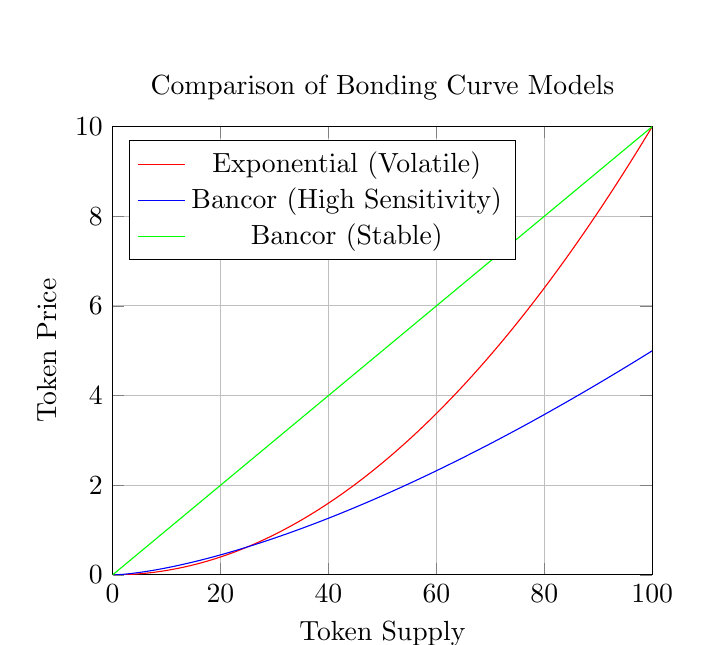
\begin{tikzpicture}
\begin{axis}[
    title={Comparison of Bonding Curve Models},
    xlabel={Token Supply},
    ylabel={Token Price},
    xmin=0, xmax=100,
    ymin=0, ymax=10,
    legend pos=north west,
    grid=major,
    samples=100,
    no markers,
]
% Exponential Curve (e.g., Memecoin)
\addplot[domain=0:100, color=red] {0.001*x^2};
\addlegendentry{Exponential (Volatile)}

% Bancor-style Curve (High Sensitivity)
\addplot[domain=0:100, color=blue] {0.005*x^1.5};
\addlegendentry{Bancor (High Sensitivity)}

% Bancor-style Curve (Low Sensitivity / Stable)
\addplot[domain=0:100, color=green] {0.1*x};
\addlegendentry{Bancor (Stable)}

\end{axis}
\end{tikzpicture}
\caption{A visual comparison of different bonding curve models. Exponential curves offer aggressive price discovery, suitable for viral assets. Bancor-style curves provide more controlled and predictable price trajectories, with stability adjustable by the project creator via parameters like the Connector Weight.}
\label{fig:bonding_curves}
\end{figure}

    \item \textbf{Decentralized AI Inference:} A forthcoming marketplace for AI computation.
    \begin{itemize}[leftmargin=*, itemsep=2pt]
        \item \textbf{Core Roles:} \textbf{Clients}, \textbf{Inference Providers}, and \textbf{Arbitrators}.
        \item \textbf{Execution Flow:} Clients submit jobs, Providers execute them, and Arbitrators verify a subset of results.
        \item \textbf{Economic Security:} Providers stake \texttt{\$SCLT}, which is subject to slashing for misbehavior.
    \end{itemize}
\end{itemize}

\hrule
\newpage
\section{Tokenomics}
The native asset of the Scarlett protocol is tentatively named \texttt{\$SCLT}.
\begin{itemize}[leftmargin=*, itemsep=2pt]
    \item \textbf{Total Supply \& Emission Schedule:} Scarlett implements a dynamic monetary policy using the Cosmos SDK \texttt{x/mint} module. At genesis, parameters like the target staking ratio (e.g., 67\%) and min/max inflation rates are set. The module automatically adjusts inflation to maintain the target ratio. All parameters are controlled by on-chain governance.
    
    \item \textbf{Token Utility:}
    \begin{enumerate}[leftmargin=*, itemsep=2pt]
        \item \textbf{Staking:} Securing the network via Proof-of-Stake.
        \item \textbf{Gas:} Paying for transaction fees.
        \item \textbf{Governance:} Voting on proposals.
        \item \textbf{Economic Bonding:} Staking to register modules/contracts.
        \item \textbf{Launchpad Collateral:} Primary asset for bonding curves.
    \end{enumerate}
    \item \textbf{A Control Theory Model for Dynamic Inflation:} The dynamic inflation mechanism can be modeled as a Proportional-Integral-Derivative (PID) controller, a concept from control theory used to maintain a system's output at a desired setpoint (the target staking ratio). The inflation rate is the actuator, adjusted to guide the actual staking ratio toward its target. The change in inflation (\(\Delta I\)) is calculated based on the deviation from the target:
    \[ \Delta I = P_{\text{term}} + I_{\text{term}} + D_{\text{term}} \]
    Where the terms are:
    \begin{itemize}
        \item \textbf{Proportional (\(P_{\text{term}}\)):} \(K_p \times (\text{Target} - \text{Actual})\). Provides an immediate response proportional to the current error.
        \item \textbf{Integral (\(I_{\text{term}}\)):} \(K_i \times \int (\text{Target} - \text{Actual}) \,dt\). Corrects for past errors.
        \item \textbf{Derivative (\(D_{\text{term}}\)):} \(K_d \times \frac{d(\text{Target} - \text{Actual})}{dt}\). Anticipates future error by reacting to its rate of change.
    \end{itemize}
    While the Cosmos SDK's \texttt{x/mint} module is primarily proportional, this PID model provides a more complete theoretical foundation. The coefficients (\(K_p, K_i, K_d\)) and inflation bounds are governance-controlled parameters.
\end{itemize}

\hrule
\vspace{1em}
\section{Genesis \& Roadmap}

\subsection{Genesis Campaign: Proof of Community}
Scarlett's fair launch is initiated by the \textbf{Proof of Community} campaign, managed by the \texttt{x/proofofcommunity} module.
\begin{itemize}[leftmargin=*, itemsep=2pt]
    \item \textbf{Eligibility \& Genesis State:} Initial participation is earned via off-chain contributions. The curated list of addresses is embedded in the genesis state.
    \item \textbf{Mechanism: The Patience Game:} Emissions per block are distributed to a reward pool, divided equally among all wallets that have \textbf{not yet claimed}. When a user claims, their wallet is removed, increasing the share for remaining participants. The formula is: 
    \[ \text{Emission per Wallet} = \frac{\text{Total Campaign Emission per Block}}{\text{Number of Unclaimed Wallets}} \]
    \item \textbf{A Formal Game-Theoretic Analysis:} The "Patience Game" can be formally modeled as a non-cooperative, multi-player "war of attrition" to prove that it selects for participants with long-term conviction.
    \begin{itemize}
        \item \textbf{Players:} A set of \(N\) eligible participants.
        \item \textbf{State at time \(t\):} The number of participants yet to claim, \(N_t\).
        \item \textbf{Reward Rate:} A constant total emission \(R\) per block is divided among remaining participants, so the rate at block \(t\) is \(r_t = R / N_t\).
        \item \textbf{Actions:} At each block, each participant can \textbf{Claim} or \textbf{Wait}.
    \end{itemize}
    The decision for a participant \(i\) at block \(t\) with accumulated rewards \(C_i(t)\) is as follows: if they \textbf{Claim}, their payoff is \(P_i^{claim} = C_i(t)\). If they \textbf{Wait}, their future payoff depends on the number of other participants who claim in the same block. The reward rate is mathematically guaranteed to increase as participants exit the game. This creates a strategic dilemma: claim an immediate, risk-free payoff or wait for a disproportionately higher future reward rate, at the risk of a decline in the token's future value. The optimal strategy depends on individual risk tolerance and time preference, but the game is explicitly designed to ensure the highest rewards flow to the most patient participants, provably selecting for a community aligned with the protocol's long-term success.
    \item \textbf{Gasless Claiming:} Claim transactions are gasless for the user, subsidized by the protocol via the Cosmos SDK's \texttt{feegrant} module.
\end{itemize}

\subsection{Roadmap}
\begin{itemize}[leftmargin=*, itemsep=2pt]
    \item \textbf{Phase 1 (Launch):} Mainnet, Proof of Community, governance, and staking.
    \item \textbf{Phase 2 (Economic Expansion):} Deployment of the Token Launchpad and DEX.
    \item \textbf{Phase 3 (Intelligence Unleashed):} Deployment of the AI Inference module.
    \item \textbf{Phase 4 (Interoperability):} IBC integration.
\end{itemize}
\vspace{1em}
\hrule
\newpage
\section{Conclusion}
Scarlett is a public good designed to support the next era of intelligent systems. By building a robust, credibly neutral, and community-governed foundation, Scarlett provides the necessary infrastructure to ensure the future of AI is open, transparent, and decentralized.

\end{document} 